% =============================================================================
%  Slides — A Comparative Study of Hard-Constrained Price-Domain Networks
%           and Native Volatility-Domain Networks for the IV Surface
% =============================================================================
\documentclass[10pt,aspectratio=169]{beamer}

\usepackage[utf8]{inputenc}
\usepackage[T1]{fontenc}
\usepackage{lmodern}
\usepackage{amsmath,amssymb}
\usepackage{booktabs}
\usepackage{graphicx}
\usepackage{subcaption}
\usepackage{tikz}
\usetikzlibrary{positioning,arrows.meta,shapes.geometric,fit,calc}

\graphicspath{{figs/}}

\usetheme{Madrid}
\usecolortheme{seahorse}
\setbeamertemplate{navigation symbols}{}
\setbeamertemplate{caption}[numbered]
\setbeamerfont{caption}{size=\scriptsize}

\newcommand{\iv}{\sigma_{\mathrm{IV}}}

\tikzset{
  block/.style  = {draw, rounded corners, thick, align=center, minimum height=0.7cm,
                   minimum width=2.0cm, fill=blue!5, font=\scriptsize},
  data/.style   = {draw, thick, align=center, minimum height=0.7cm,
                   minimum width=1.8cm, fill=yellow!15, font=\scriptsize},
  model/.style  = {draw, rounded corners, thick, align=center, minimum height=0.8cm,
                   minimum width=2.2cm, fill=green!8, font=\scriptsize},
  hyper/.style  = {draw, rounded corners, thick, align=center, minimum height=0.8cm,
                   minimum width=2.2cm, fill=purple!8, font=\scriptsize},
  arrow/.style  = {-Stealth, thick},
}

\title[IV Surface: Price vs Vol Domain]{Hard Price-Domain Constraints vs.\ Native Volatility-Domain Models for the IV Surface}
\subtitle{An Empirical Comparison of ISNN, HyperIV, HyperISNN and SSVI}
\author[Parshv Joshi]{Parshv Joshi}
\institute[]{\small Under the mentorship of Prof.\ Abhishek Tilva}
\date[April 2026]{April 2026}

\begin{document}

% ============================================================
\begin{frame}
\titlepage
\end{frame}

% ============================================================
\begin{frame}{Outline}
\tableofcontents
\end{frame}

% ============================================================
\section{Motivation \& Objective}

\begin{frame}{Motivation}
The implied-volatility (IV) surface $\iv(K, T)$ is the central object of equity derivatives modelling.\medskip

Three communities have produced largely \textbf{non-overlapping literatures}:
\begin{itemize}
  \item \textbf{Parametric arbitrage-free} models (SVI / SSVI). Robust, but a fresh non-convex fit per day.
  \item \textbf{Hard-constrained price-domain neural surrogates} (ISNN). Arbitrage-free by construction.
  \item \textbf{Volatility-domain hyper-networks} (HyperIV). Train once across years; per-day inference is a single forward pass.
\end{itemize}\medskip

\textbf{Question.} Nobody has compared these on the same data, the same evaluation, the same arbitrage filter. This work does.
\end{frame}

\begin{frame}{Objectives}
\begin{enumerate}
  \item Build one reproducible pipeline: raw OptionMetrics SPX EOD $\to$ Moussa filter $\to$ unified quote store.
  \item Implement four pipelines under one harness:
    \begin{itemize}\small
      \item[A.] ISNN-2 (per-day, price domain) --- \textit{Jadoon et al., 2025}
      \item[B.] HyperIV (amortised, IV domain) --- \textit{Yang et al., 2025}
      \item[C.] HyperISNN (novel, residual hyper-net for ISNN weights)
      \item[D.] SSVI (per-day parametric) --- \textit{Gatheral \& Jacquier, 2014}
    \end{itemize}
  \item Phase-1 (same-day fit) and Phase-2 (next-day predict via VolGAN) on the same test split.
  \item Wall-clock comparison: per-day fit vs.\ amortised inference.
\end{enumerate}
\end{frame}

% ============================================================
\section{Literature}

\begin{frame}{Literature study (the four papers we build on)}
\begin{itemize}
  \item \textbf{Moussa (2025).} Real-time LP-based arbitrage filter. Removes the minimal set of mid-quotes that violate intrinsic / calendar / butterfly bounds. We use it as the \emph{only} cleaning step.
  \item \textbf{Jadoon et al.\ (2025) --- ISNN-2.} Two-branch Input-Specified Neural Net; strictly-positive weights (softplus) make the price surface convex in $K$ and monotone in $T$ \emph{by construction}.
  \item \textbf{Yang et al.\ (2025) --- HyperIV.} Set-Transformer encoder $g_\theta(Z_t) \to \omega_t \in \mathbb{R}^{337}$, which weights a tiny IV-MLP $h_{\omega_t}(k, T) \to \iv$. Trained once with MSE(IV) + soft arbitrage penalties.
  \item \textbf{Gatheral \& Jacquier (2014) --- SSVI.} Five-parameter total-variance surface with analytical no-arbitrage inequalities on $(\rho, \eta, c)$.
\end{itemize}
\medskip
\scriptsize Other references (VolGAN, Set Transformer, ICNN, Hypernetworks, Roper, Durrleman, $\dots$) are listed in the paper.
\end{frame}

% ============================================================
\section{Technical Details}

\begin{frame}{End-to-end pipeline}
\centering
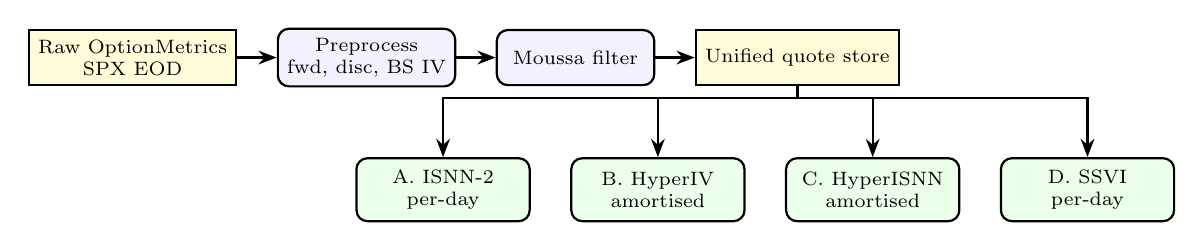
\begin{tikzpicture}[node distance=0.4cm and 0.5cm]
  \node[data]  (raw)   {Raw OptionMetrics \\ SPX EOD};
  \node[block, right=of raw] (pre) {Preprocess \\ \scriptsize fwd, disc, BS IV};
  \node[block, right=of pre] (mou) {Moussa filter};
  \node[data,  right=of mou] (uni) {Unified quote store};
  \draw[arrow] (raw) -- (pre); \draw[arrow] (pre) -- (mou); \draw[arrow] (mou) -- (uni);

  \node[model, below=0.9cm of uni, xshift=-4.5cm] (A) {A. ISNN-2 \\ \scriptsize per-day};
  \node[model, right=of A] (B) {B. HyperIV \\ \scriptsize amortised};
  \node[model, right=of B] (C) {C. HyperISNN \\ \scriptsize amortised};
  \node[model, right=of C] (D) {D. SSVI \\ \scriptsize per-day};
  \draw[arrow] (uni.south) -- ++(0,-0.15) -| (A.north);
  \draw[arrow] (uni.south) -- ++(0,-0.15) -| (B.north);
  \draw[arrow] (uni.south) -- ++(0,-0.15) -| (C.north);
  \draw[arrow] (uni.south) -- ++(0,-0.15) -| (D.north);
\end{tikzpicture}
\medskip
\begin{itemize}\small
  \item \textbf{Dataset.} 1\,762 SPX trading days, 2013-01 -- 2019-12. Train 2013--17, Val 2018, Test 2019.
  \item \textbf{Phase-1.} Same-day fit error in IV and \$ price.
  \item \textbf{Phase-2.} Next-day surface generated by VolGAN, scored against realised market.
\end{itemize}
\end{frame}

\begin{frame}{Pipeline A --- ISNN-2 (per-day, price domain)}
\begin{columns}[T,onlytextwidth]
\begin{column}{0.55\linewidth}
\begin{itemize}\small
  \item Two-branch net on $(x_0, t_0) = (K/F, T)$.
  \item Strictly-positive weights $W^{xx}, W^{xt}, W^{tt}$ via softplus + clamp.
  \item Output: normalized call $C/S$, \emph{convex in $K$, monotone in $T$ by construction}.
  \item \textbf{Loss:} MSE on $C/S$.
  \item \textbf{Train:} Adam, LR $10^{-2}$, 2{,}000 epochs \emph{per day}.
  \item Hard arbitrage guarantee, no soft penalties needed.
\end{itemize}
\end{column}
\begin{column}{0.45\linewidth}
\centering
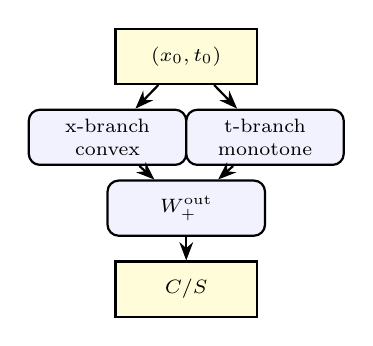
\begin{tikzpicture}[node distance=0.3cm and 0.4cm]
  \node[data] (in) {$(x_0, t_0)$};
  \node[block, below=of in, xshift=-1.0cm] (xb) {x-branch \\ \scriptsize convex};
  \node[block, below=of in, xshift=1.0cm]  (tb) {t-branch \\ \scriptsize monotone};
  \node[block, below=1.2cm of in] (out) {$W^{\mathrm{out}}_+$};
  \node[data,  below=of out] (y) {$C/S$};
  \draw[arrow] (in) -- (xb); \draw[arrow] (in) -- (tb);
  \draw[arrow] (xb) -- (out); \draw[arrow] (tb) -- (out);
  \draw[arrow] (out) -- (y);
\end{tikzpicture}
\end{column}
\end{columns}
\end{frame}

\begin{frame}{Pipeline B --- HyperIV (amortised, IV domain)}
\centering
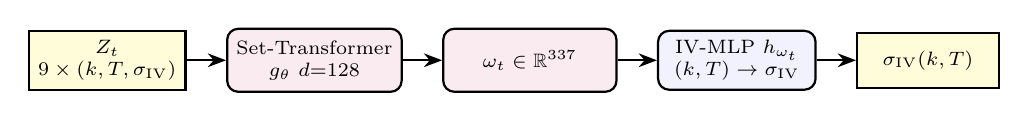
\begin{tikzpicture}[node distance=0.3cm and 0.5cm]
  \node[data] (Z) {$Z_t$ \\ \scriptsize $9\times(k,T,\iv)$};
  \node[hyper, right=of Z] (enc) {Set-Transformer \\ $g_\theta$ \scriptsize $d{=}128$};
  \node[hyper, right=of enc] (om) {$\omega_t \in \mathbb{R}^{337}$};
  \node[block, right=of om] (h) {IV-MLP $h_{\omega_t}$ \\ \scriptsize $(k,T)\to\iv$};
  \node[data, right=of h] (sig) {$\iv(k, T)$};
  \draw[arrow] (Z) -- (enc); \draw[arrow] (enc) -- (om); \draw[arrow] (om) -- (h); \draw[arrow] (h) -- (sig);
\end{tikzpicture}
\medskip
\begin{itemize}\small
  \item Set-Transformer encoder ($d{=}128$, $2$ heads, $2$ layers) over a $9$-element reference set $Z_t$.
  \item \textbf{Loss:} MSE($\iv$) + calendar / butterfly ($g$-fn) / Durrleman soft arbitrage penalties.
  \item \textbf{Train:} Adam $10^{-3}$, batch $128$, $500$ epochs, cosine $\to 10^{-5}$ --- \emph{trained once on 2013--2017}.
  \item \textbf{Inference:} one forward pass through $g_\theta$, then any number of $h_{\omega_t}$ queries.
  \item Reference set: positive call deltas $\{0.75, 0.50, 0.25\}$ at $3$ short and $3$ long maturities.
\end{itemize}
\end{frame}

\begin{frame}{Pipeline C --- HyperISNN (novel, residual hyper-net for ISNN weights)}
\centering
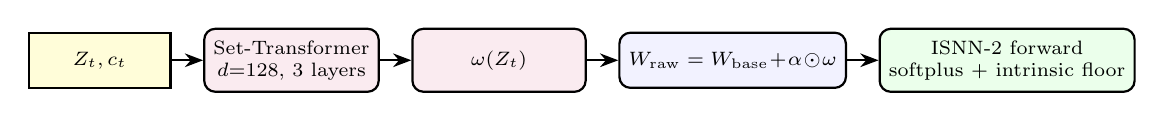
\begin{tikzpicture}[node distance=0.3cm and 0.4cm]
  \node[data] (Z) {$Z_t, c_t$};
  \node[hyper, right=of Z] (enc) {Set-Transformer\\ $d{=}128$, 3 layers};
  \node[hyper, right=of enc] (om) {$\omega(Z_t)$};
  \node[block, right=of om] (mix) {$W_{\mathrm{raw}} = W_{\mathrm{base}}\!+\!\alpha\!\odot\!\omega$};
  \node[model, right=of mix] (isnn) {ISNN-2 forward \\ \scriptsize softplus + intrinsic floor};
  \draw[arrow] (Z) -- (enc); \draw[arrow] (enc) -- (om); \draw[arrow] (om) -- (mix); \draw[arrow] (mix) -- (isnn);
\end{tikzpicture}
\medskip
\begin{itemize}\small
  \item \textbf{Residual scheme.} Per day: $W_{\mathrm{raw}} = W_{\mathrm{base}} + \alpha \odot \omega(Z_t, c_t)$, then softplus on positive entries. $W_{\mathrm{base}}$ \& $\alpha$ shared across all days.
  \item \textbf{Hard intrinsic floor.} Forward-measure bound $\max(0, 1{-}m)$ added \emph{inside} the ISNN forward pass.
  \item \textbf{Two-phase training.} 500 warm-up steps with $\alpha$ \& hyper-net frozen ($W_{\mathrm{base}}$ + $b^{\mathrm{out}}$ only); then full joint training for 9{,}500 more steps.
  \item \textbf{Optimizer.} AdamW $3{\times}10^{-4}$, wd $10^{-4}$, batch $32$, cosine warm restart $T_0{=}1000$, grad clip $1$.
  \item Available losses: MSE / Vega-MSE / Huber / log-price / Huber+Vega hybrid (paper uses MSE).
\end{itemize}
\end{frame}

\begin{frame}{Pipeline D --- SSVI (per-day parametric)}
\begin{itemize}\small
  \item Gatheral \& Jacquier (2014) total-variance surface:
  \[
    w(k, t) = \tfrac{\theta(t)}{2}\Big(1 + \rho\, \phi\, k + \sqrt{(\phi k + \rho)^2 + (1 - \rho^2)}\Big),
    \quad \phi(\theta) = \eta / \sqrt{\theta},
    \quad \theta(t) = a + b\, t^c.
  \]
  \item Five free parameters $(a, b, c, \eta, \rho)$ per day.
  \item \textbf{Fit.} ATM-weighted MSE on $\iv$ via L-BFGS-B with \emph{$10$ random restarts}.
  \item \textbf{Constraints.} Box constraints + Gatheral--Jacquier inequalities $\Rightarrow$ surface is butterfly- and calendar-arbitrage-free.
  \item Strong baseline: small parameter count, tight inductive bias.
\end{itemize}
\end{frame}

% ============================================================
\section{Results}

\begin{frame}{Headline IV-domain results (Test 2019)}
\centering
\small
\begin{tabular}{lcccc}
\toprule
& \multicolumn{2}{c}{Phase-1 (same-day)} & \multicolumn{2}{c}{Phase-2 (next-day VolGAN)} \\
\cmidrule(lr){2-3}\cmidrule(lr){4-5}
Pipeline & RMSE & MAE & RMSE & MAE \\
\midrule
A. ISNN       & $0.0737$ & $0.0564$ & $0.0644$ & $0.0500$ \\
B. HyperIV    & $0.0131$ & $0.0091$ & $0.0170$ & $0.0131$ \\
C. HyperISNN  & $0.0865$ & $0.0686$ & $0.0722$ & $0.0593$ \\
D. SSVI       & $\mathbf{0.0077}$ & $\mathbf{0.0048}$ & $\mathbf{0.0174}$ & $\mathbf{0.0122}$ \\
\bottomrule
\end{tabular}
\medskip
\begin{itemize}\small
  \item SSVI wins Phase-1 by a wide margin; HyperIV second.
  \item HyperIV essentially ties SSVI on Phase-2 --- without ever seeing the test day at training time.
  \item ISNN / HyperISNN are an order of magnitude worse in IV.
\end{itemize}
\end{frame}

\begin{frame}{Headline price-domain results}
\centering
\small
\begin{tabular}{lcccc}
\toprule
Pipeline & \$ RMSE & \$ MAE & Rel-MAE & N quotes \\
\midrule
A. ISNN \scriptsize (native)        & $16.30$ & $13.02$ & $4.91$  & $153{,}777$ \\
B. HyperIV \scriptsize (BS-priced)  & $3.51$  & $2.12$  & $0.25$  & $153{,}777$ \\
C. HyperISNN \scriptsize (native)   & $26.52$ & $18.15$ & $2.18$  & $153{,}777$ \\
D. SSVI \scriptsize (BS-priced)     & $\mathbf{2.35}$  & $\mathbf{1.24}$  & $\mathbf{0.12}$  & $153{,}777$ \\
\bottomrule
\end{tabular}
\medskip
\begin{itemize}\small
  \item Native price-domain models (A, C) are $5\times$--$10\times$ worse \emph{in their own domain} than IV-domain models that go through a BS inversion.
\end{itemize}
\end{frame}

\begin{frame}{Why does the price-domain model lose in price?}
\textbf{Moneyness asymmetry of MSE on normalized prices.}
\begin{itemize}\small
  \item Deep ITM: $C_{\mathrm{norm}} \to 1$ (mostly intrinsic value, no information).
  \item Deep OTM: $C_{\mathrm{norm}} \to 0$ (all the volatility skew lives here).
  \item MSE over-weights intrinsic value, under-weights skew.
  \item A ``small'' relative error on a deep ITM normalized price $\Rightarrow$ a \emph{large dollar} error after multiplying back by spot.
\end{itemize}
\medskip
\textbf{IV is on a common scale} ($\sim 0.1$--$0.8$): MSE on IV implicitly equalises every contract. BS pricing then yields small \$ errors uniformly.\medskip

\textbf{Practical corollary.} If you must use ISNN for the architectural arbitrage guarantee, do not read \$ off the price head --- invert to IV and re-price.
\end{frame}

\begin{frame}{Visual evidence: price-domain surfaces (ISNN, HyperISNN)}
\centering
\begin{tabular}{cc}
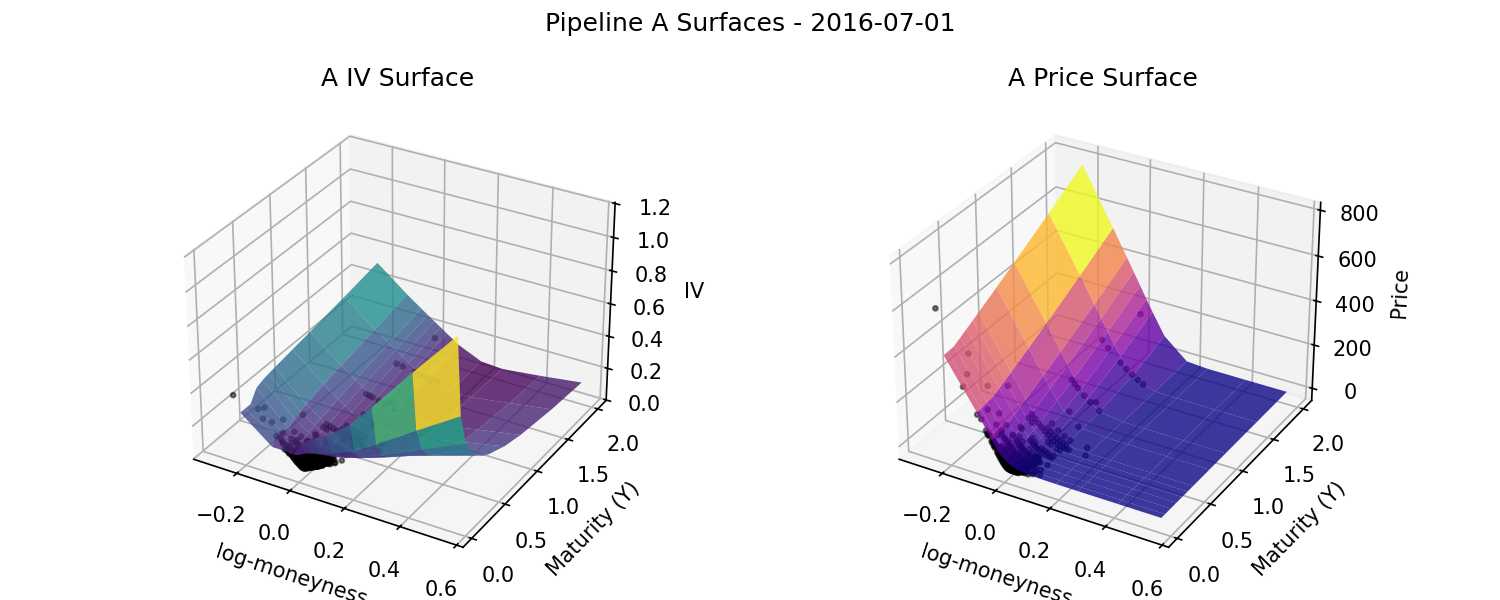
\includegraphics[height=0.62\textheight]{09_3d_surfaces_A.png} &
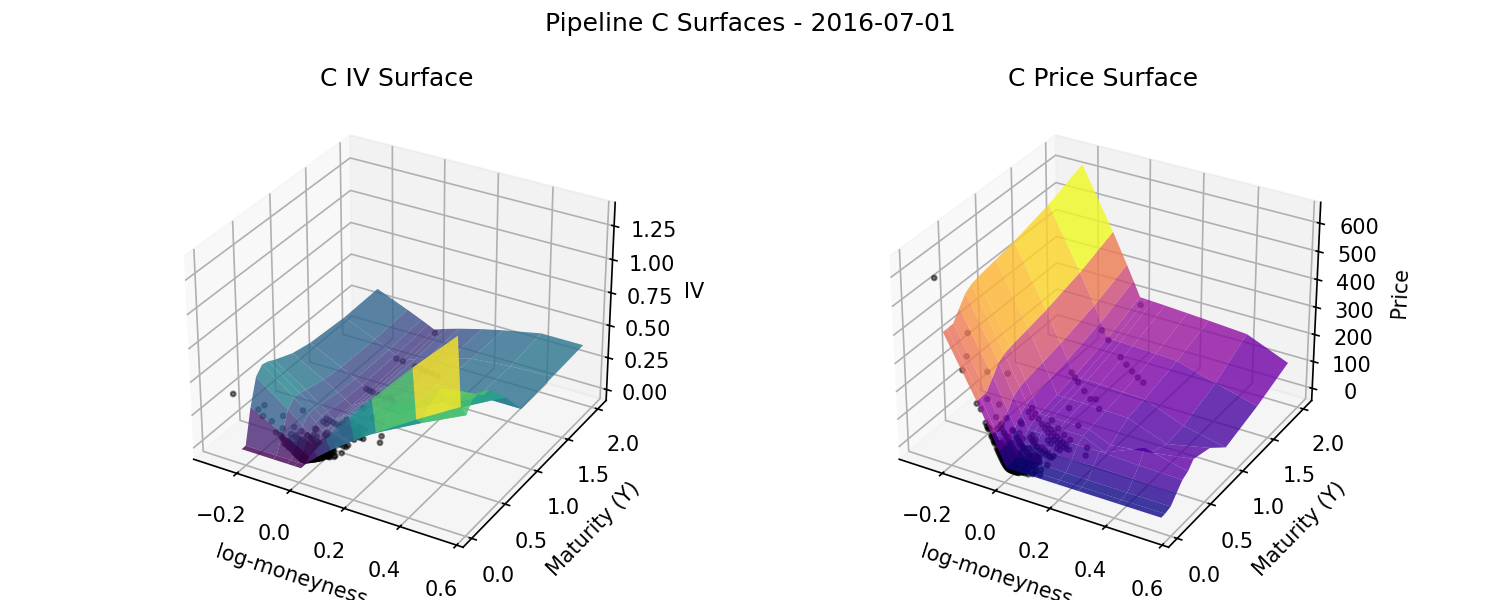
\includegraphics[height=0.62\textheight]{09_3d_surfaces_C.png} \\
\small A. ISNN & \small C. HyperISNN
\end{tabular}\medskip

\small ISNN / HyperISNN: \emph{over-smoothed wings}; butterfly-strict positivity limits surface flexibility, so the smile collapses towards the centre.
\end{frame}

\begin{frame}{Visual evidence: IV-domain surfaces (HyperIV, SSVI)}
\centering
\begin{tabular}{cc}
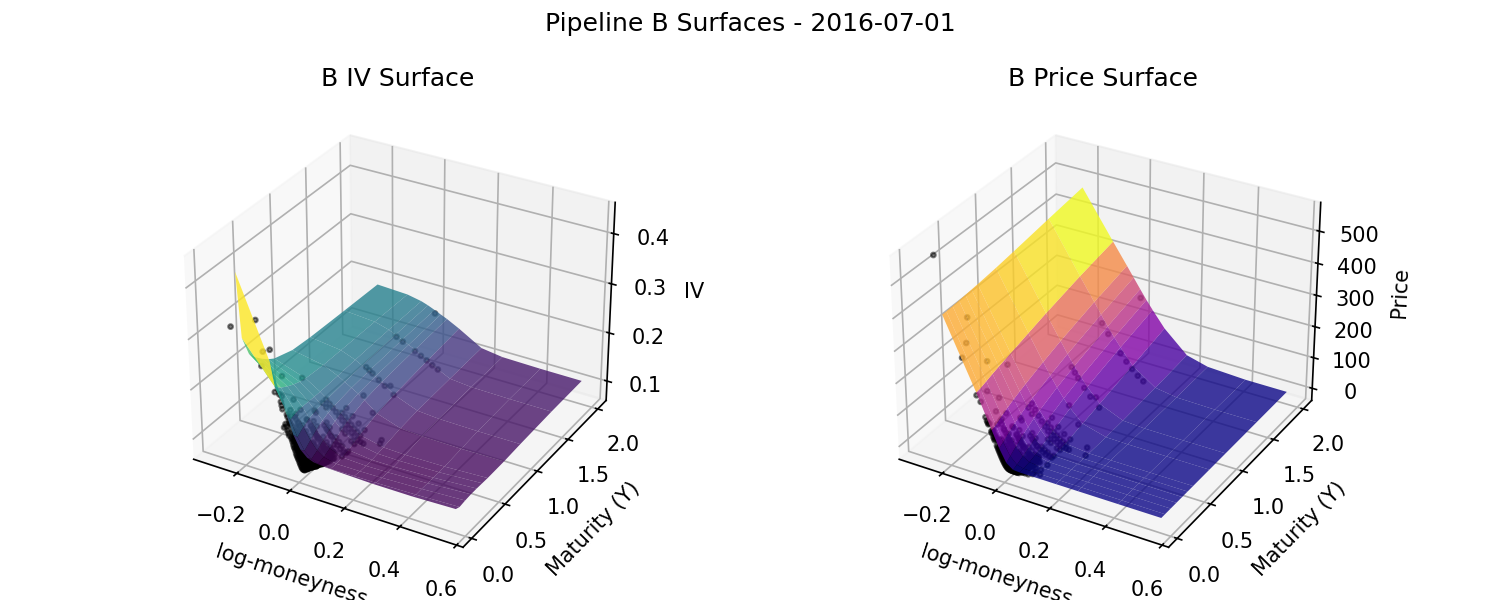
\includegraphics[height=0.62\textheight]{09_3d_surfaces_B.png} &
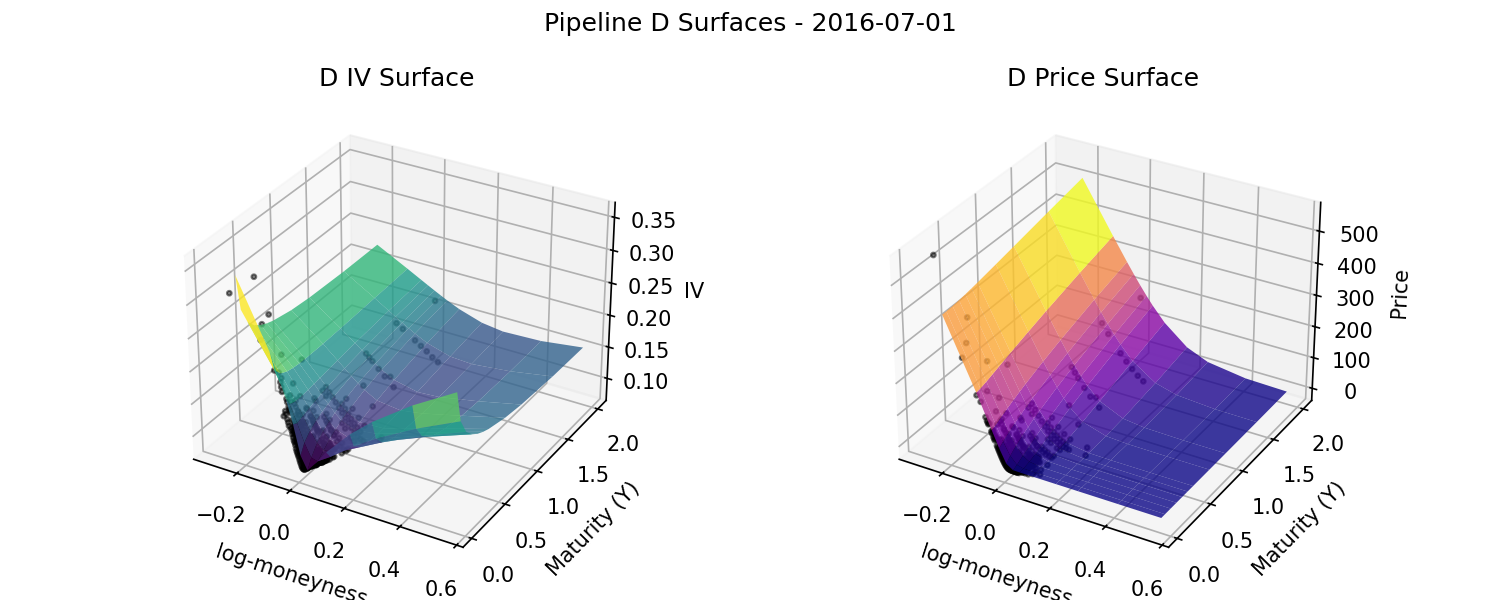
\includegraphics[height=0.62\textheight]{09_3d_surfaces_D.png} \\
\small B. HyperIV & \small D. SSVI
\end{tabular}\medskip

\small HyperIV / SSVI: \emph{tight, well-skewed} surfaces that match the SPX smile and term structure. Compare against the previous slide --- same axis ranges, the wings are clearly there.
\end{frame}

\begin{frame}{Diagnostics: slices and rolling RMSE}
\centering
\begin{tabular}{cc}
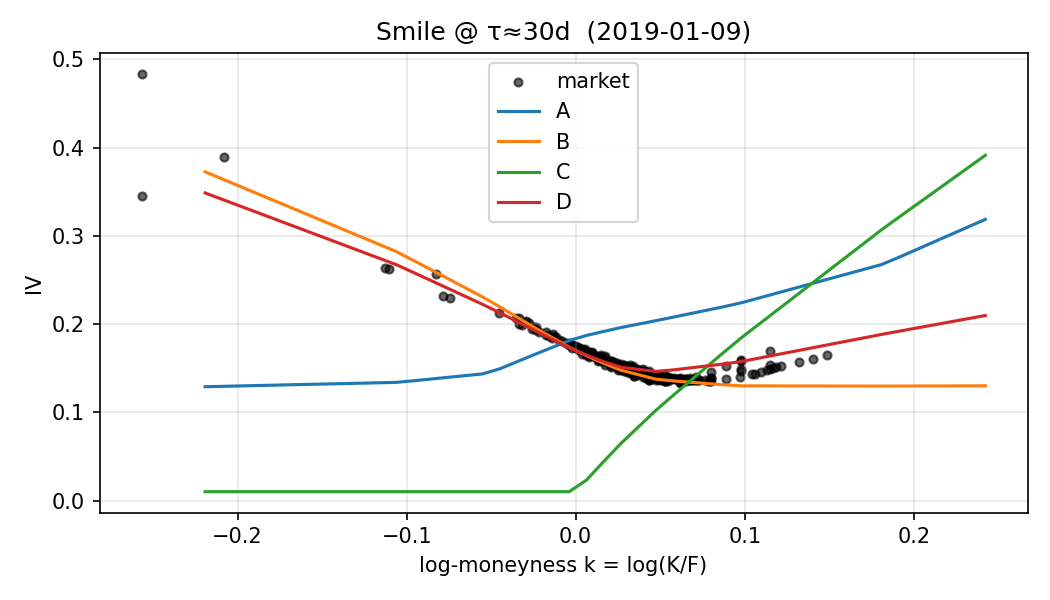
\includegraphics[width=0.42\linewidth]{slice_smile_2019-01-09.png} &
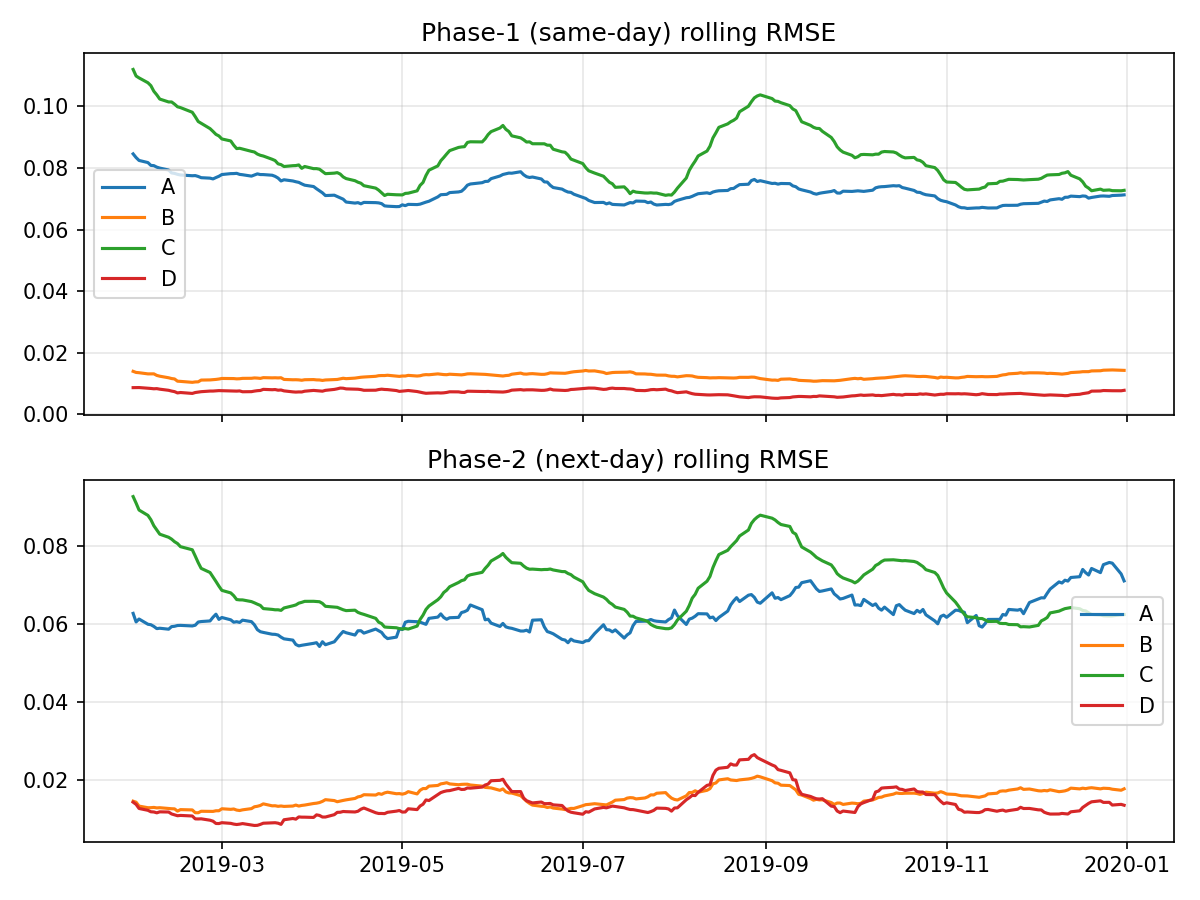
\includegraphics[width=0.45\linewidth]{06_rolling_rmse.png} \\
\scriptsize Smile slice 2019-01-09 & \scriptsize Rolling RMSE through 2019
\end{tabular}\bigskip

SSVI dominates uniformly; HyperIV competitive everywhere; price-domain pipelines miss the wings.
\end{frame}

\begin{frame}{Wall-clock: HyperIV inference vs.\ SSVI per-day fit}
\centering
\small
\begin{tabular}{lrr}
\toprule
Operation (single-thread, M-series CPU) & median (ms / day) & p95 (ms / day) \\
\midrule
SSVI per-day fit (L-BFGS-B, $10$ restarts)              & $154.5$ & $241.6$ \\
HyperIV: encoder ($g_\theta(Z_t)\!\to\!\omega_t$)       & $0.147$ & $0.604$ \\
HyperIV: encoder + market-quote evaluation              & $0.282$ & $1.067$ \\
\bottomrule
\end{tabular}\medskip

\begin{itemize}\small
  \item Median speedup HyperIV vs.\ SSVI: $\mathbf{\approx 547\times}$.
  \item This is the central operational case for hyper-networks in finance: amortise calibration, then price on the margin in microseconds.
  \item Reproduced by \texttt{python bench\_timing.py} in the repo.
\end{itemize}
\end{frame}

\begin{frame}{HyperISNN vs.\ ISNN}
\textbf{Less accurate.}
\begin{itemize}\small
  \item Phase-1 IV RMSE: $0.0865$ vs.\ ISNN's $0.0737$.
  \item Phase-1 \$ RMSE: $26.5$ vs.\ ISNN's $16.3$.
  \item Cause: a single shared $W_{\mathrm{base}}$ + per-parameter $\alpha$ cannot match a freshly-fit ISNN; the warm-up ``mean ISNN'' basin is too restrictive.
\end{itemize}
\medskip
\textbf{Much faster.}
\begin{itemize}\small
  \item Inherits HyperIV's amortised inference.
  \item Trades $\sim 15\%$ relative IV accuracy for two-to-three orders of magnitude in inference cost vs.\ per-day ISNN.
\end{itemize}
\medskip
\textbf{Lesson.} The hyper-network template is portable to hard-constrained price-domain nets, but the cost in accuracy outweighs the speed gain when an IV-domain alternative (HyperIV) is available.
\end{frame}

\begin{frame}{Phase-2: better Phase-1 = better next-day forecast}
\centering
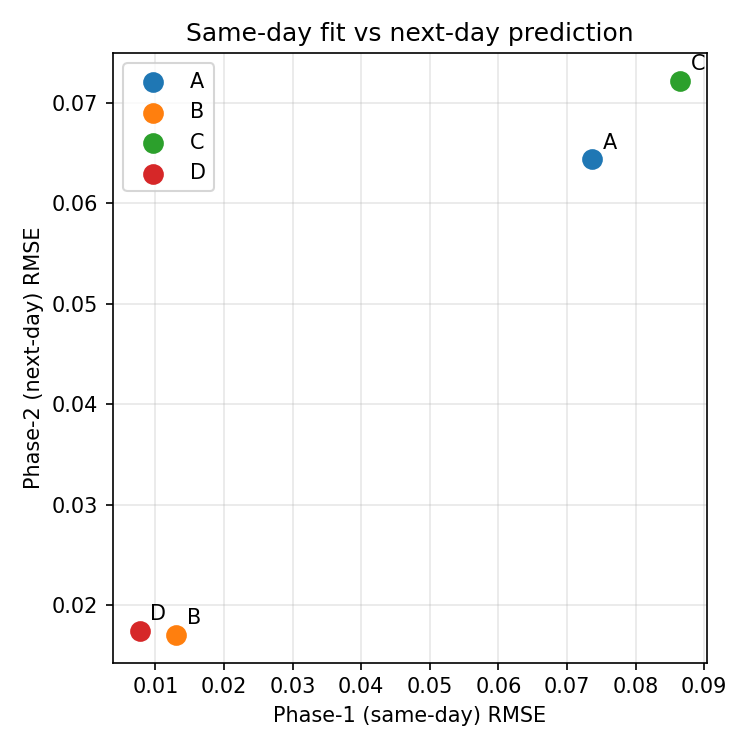
\includegraphics[width=0.55\linewidth]{02_p1_vs_p2_scatter.png}\medskip

\begin{itemize}\small
  \item VolGAN is \emph{not} a regulariser. Whatever errors live in the Phase-1 surface are absorbed and propagated.
  \item The Phase-2 ranking is the same as the Phase-1 ranking: SSVI $\preceq$ HyperIV $\ll$ ISNN $\le$ HyperISNN.
  \item Trivial but worth stating: don't expect a downstream generator to compensate for an inaccurate surface.
\end{itemize}
\end{frame}

% ============================================================
\section{Summary}

\begin{frame}{Final outcome --- five takeaways}
\begin{enumerate}\small
  \item \textbf{Native price-domain hard-constrained nets (ISNN, HyperISNN) underperform IV-domain models (HyperIV, SSVI)} on every metric, including their own \$ domain.
  \item \textbf{SSVI wins Phase-1.} Five parameters with hard inequalities is hard to beat; cost is $\sim$$160$\,ms per-day fit.
  \item \textbf{HyperIV essentially matches SSVI on Phase-2 and is $\sim 500\times$ faster at inference.} The case for amortised hyper-networks in finance.
  \item \textbf{HyperISNN trades accuracy for speed in the price-domain family.} Useful template, but worse than ISNN on accuracy.
  \item \textbf{Better Phase-1 surfaces $\Rightarrow$ better Phase-2 forecasts.} VolGAN does not save you.
\end{enumerate}\medskip

\textbf{Recommendation.} For batch backtests / intraday re-pricing: use HyperIV. For one-off per-day calibration with no latency budget: use SSVI. Avoid native ISNN price outputs in production.
\end{frame}

% ============================================================
\section{References}

\begin{frame}{Main references}
\footnotesize
\begin{itemize}
  \item \textbf{Yang, Chen, Shu, Hospedales, Pun (2025).} HyperIV: Real-time Implied Volatility Smoothing via Hypernetworks. \textit{ICML 2025.}
  \item \textbf{Jadoon, Yu, Ng, Liu (2025).} Input Specified Neural Networks for Arbitrage-Free Volatility Surface Modeling. \textit{arXiv:2503.00268.}
  \item \textbf{Gatheral \& Jacquier (2014).} Arbitrage-Free SVI Volatility Surfaces. \textit{Quantitative Finance, 14(1):59--71.}
  \item \textbf{Moussa (2025).} Arbitrage Filtering of Option Prices: A Simple Real-Time Approach. \textit{Working paper.}
\end{itemize}\medskip
\centering \emph{Full reference list (VolGAN, Set Transformer, ICNN, HyperNetworks, Roper, Durrleman, Corbetta et al., \dots) is in the paper.}
\end{frame}

\begin{frame}
\centering
\Huge Thank you. \\[0.5em]
\large Questions?
\end{frame}

\end{document}
